%!TEX TS-program = xelatex  
%!TEX encoding = UTF-8 Unicode  

\documentclass[11pt]{beamer}                                                                                                                                    
\usepackage{beamerthemesplit}
\usepackage{amsmath}
\usepackage{amsfonts}
\usepackage{amssymb}
\usepackage{latexsym}
\usepackage{ctex}
\usepackage{makeidx}
\usepackage{graphicx}
\usepackage{float}
\usepackage{color}
\usepackage{pst-grad} % For gradients
\usepackage{pst-plot} % For axes  
\usetheme{Madrid}  
\usecolortheme{beaver}
%\usefonttheme{serif}
%用于设置定理、定义等格式的宏包
\usepackage{flushend, cuted} %

\usepackage{indentfirst,latexsym,bm}
\usepackage{amsmath,amssymb,amsfonts}
\usepackage{pifont} 
\usepackage{fontspec,xltxtra,xunicode}  
\defaultfontfeatures{Mapping=tex-text} 
\usepackage[noend, ruled, linesnumbered]{algorithm2e}
\setromanfont{宋体} %设置中文字体  
\XeTeXlinebreaklocale “zh”  
\XeTeXlinebreakskip = 0pt plus 1pt minus 0.1pt %文章内中文自动换行  

\newfontfamily{\H}{黑体} 
\newfontfamily{\E}{Arial} 
\newfontfamily{\TNR}{Times New Roman} 

\usepackage[english]{babel}  
\usepackage{times}  
\usepackage[T1]{fontenc} 
\setbeamertemplate{caption}[numbered]
\setbeamertemplate{footline}[frame number]%页码
\setbeamertemplate{navigation symbols}{}
\setbeamertemplate{footline}{%
  \leavevmode%
  \hbox{%
    \begin{beamercolorbox}[wd=.45\paperwidth,ht=2.25ex,dp=1ex,center]{bg=white}%
      \usebeamerfont{author in head/foot}~
\includegraphics[height=20pt]{logo/gea.eps}
~
\includegraphics[height=20pt]{logo/enac.eps}
~
\includegraphics[height=20pt]{logo/isae-ensma.eps}
~
\includegraphics[height=20pt]{logo/isae.eps}
~
\includegraphics[height=20pt]{logo/cauc.eps}
    \end{beamercolorbox}%
    \begin{beamercolorbox}[wd=.35\paperwidth,ht=2.25ex,dp=1ex,center]{title in head/foot}%
      \usebeamerfont{title in head/foot}{基于深度残差网络的国际金价预测研究}
    \end{beamercolorbox}%
    \begin{beamercolorbox}[wd=.2\paperwidth,ht=2.25ex,dp=1ex,right]{date in head/foot}%
      \usebeamerfont{date in head/foot}\hspace*{2em}
      \insertframenumber{} / \inserttotalframenumber\hspace*{2ex}
    \end{beamercolorbox}}%
  \vskip0pt%
}

\usepackage{algorithm}             
\usepackage{algorithmic}  
\DeclareMathOperator*{\argmin}{argmin}      


%\setlength\abovecaptionskip{-7pt}
 
\title{\youyuan 基于深度残差网络的国际金价预测研究\\The Study of International Gold Price Forecasting Based on Deep Residual Network}
\institute{中国民航大学\\中欧航空工程师学院}
\author{{\footnotesize{汤吉~~121143325}\\指导老师: {\CJKfamily{zhyou} 张鸿燕~~博士}}}

%\date{\today}
\date{2016 年 06 月 06 日}
\begin{document}
\frame{\titlepage}
\begin{frame}<beamer>
\frametitle{目录}
\tableofcontents[hideallsubsections]
\end{frame}
\renewcommand\figurename{图}    
\renewcommand{\tablename}{表}


\section{课题研究背景}
\frame{
\frametitle{课题研究背景}
\begin{columns}
\column{7cm}
\begin{alertblock}{国际黄金价格}
经济全球化:复杂性,不稳定性;\\传统经济学理论的局限性;\\有效市场假说、分型市场假说;\\......
\end{alertblock}
\begin{alertblock}{深度学习网络}
层数越高,对数据的“理解”越“深”;\\梯度发散和精度下降;\\深度残差网络;\\......
\end{alertblock}
\column{5cm}







\end{columns}
}

\section{国际金价可预测性分析}

\frame {
\frametitle{R/S分析法}
Hurst指数是用来量化时间序列的自相关能力的。设有一个长度为n的时间序列,则其Hurst值$H$的原始定义为:
\begin{equation}
	E[\frac{R(n)}{S(n)}]\sim Cn^H~~~~~n\rightarrow\infty
\end{equation}
其中R(n)为这n个值的极差,S(n)是它们的标准差,E表示求期望,C是一个常数。\\
\begin{alertblock}{Hurst指数的含义}
\begin{enumerate}
\item  $0.5< H \le 1$ - 序列具有一定的保持趋势的能力;
\item $0\le H < 0.5$ - 序列相邻的值会不断在高值和低值之间切换。
\end{enumerate}
\end{alertblock}
}


\frame {
\frametitle{R/S分析法}
\begin{alertblock}{对照组设置}
\begin{enumerate}
\item 我们选择2001年1月2日至2014年12月31日时间段的国际金价走势,称为实际金价走势。
\item 实际金价进行小于30交易日滤波之后加上均值为0,方差为当日金价3\%的高斯白噪声,得到随机模拟金价。
\end{enumerate}
\end{alertblock}
\vspace{-2em}
\begin{figure}
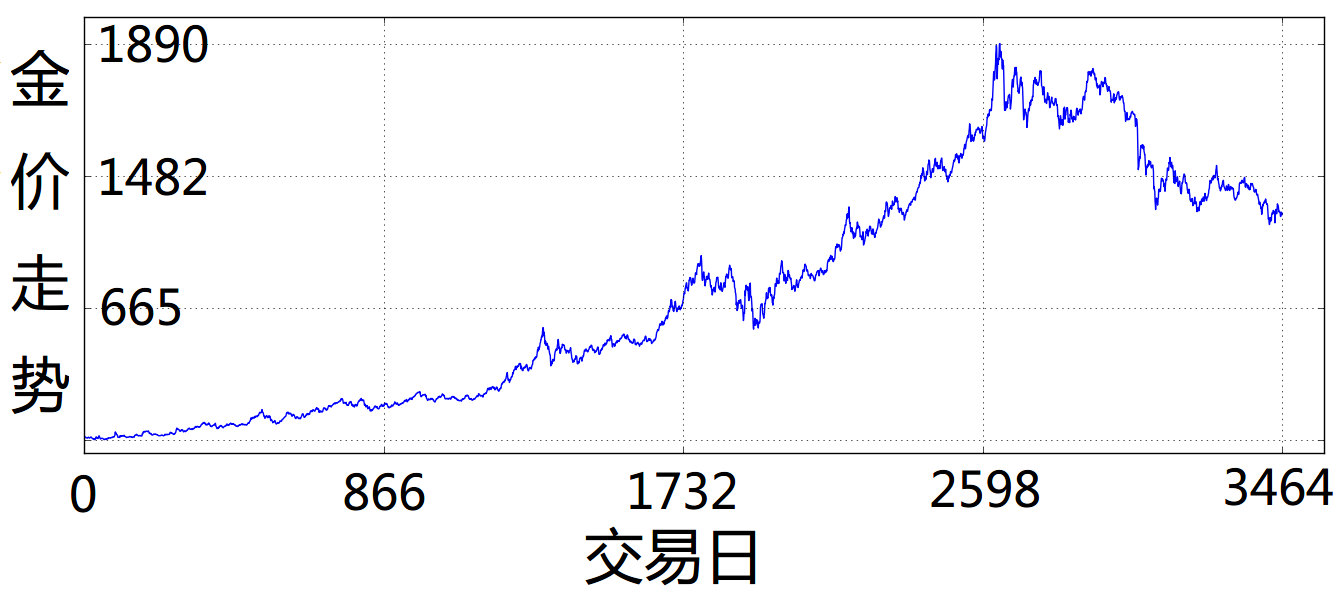
\includegraphics[height=2.8cm]{pic/1_1.png} 
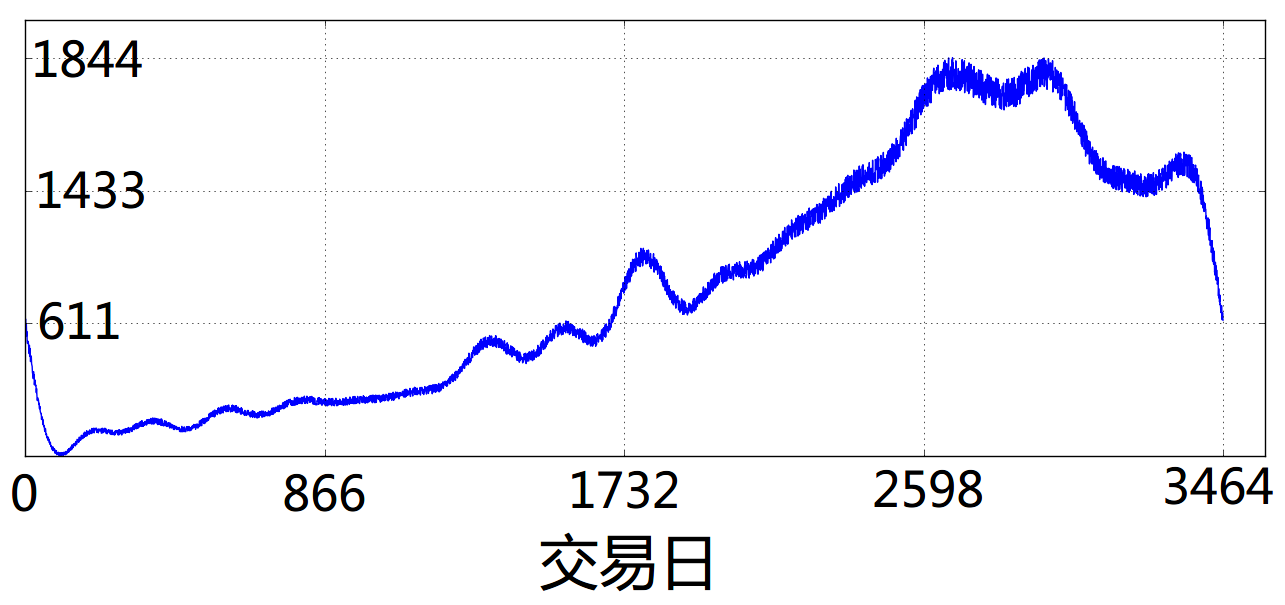
\includegraphics[height=2.8cm]{pic/1_2.png}	
\vspace{-1em}
\caption{实际金价走势(左)与随机模拟金价走势(右)}
\vspace{-1em}
\end{figure}
}


\frame {
\frametitle{R/S分析法}
我们以实际金价(蓝色)与随机模拟金价(绿色)以10交易日为基础,计算每交易日对应的Hurst指数(H)。
\begin{figure}
\vspace{-0.2em}
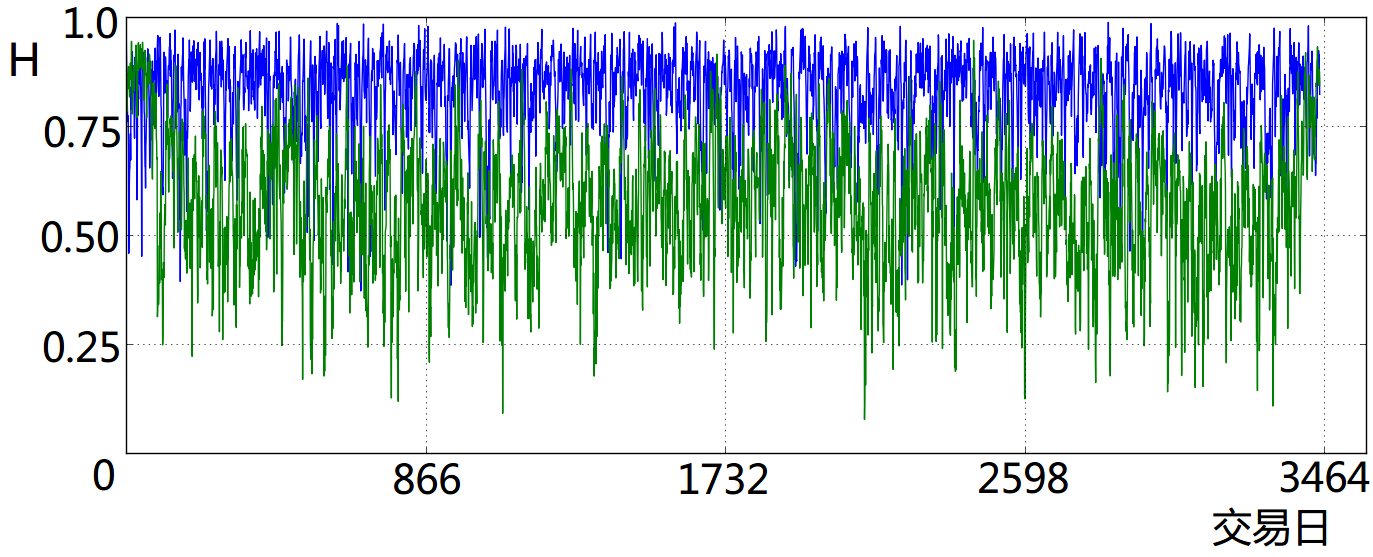
\includegraphics[width=4.3in]{pic/2.png}	
\vspace{-1em}
\caption{实际金价走势(蓝)与随机模拟金价走势(绿)Hurst指数对比}
\end{figure}
}





\frame {
\frametitle{国际金价预测流程}
\begin{figure}
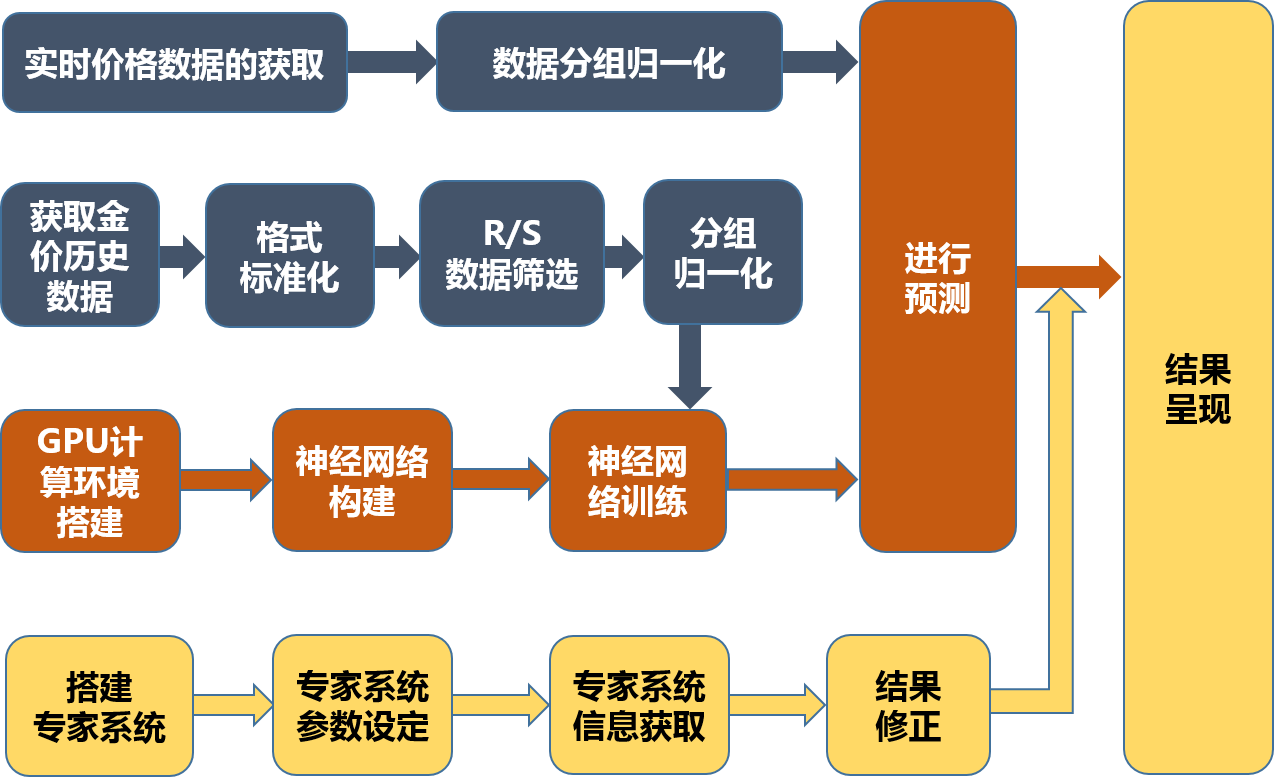
\includegraphics[height=6cm,width=4in]{pic/3.png}
\vspace{-1em}
\caption{国际金价预测流程图}
\end{figure}
}



\section{深度残差网络}
\subsection{深度残差网络简介}
\frame {
\frametitle{深度学习}
假设有一个输入$Input$经过系统$\{S_1,…,S_n \}$得到输出 $Output$ ,可以将这个过程$ Input \rightarrow S_1\rightarrow S_2\rightarrow ...\rightarrow S_n  \rightarrow Output$ 表示为:
\begin{figure}
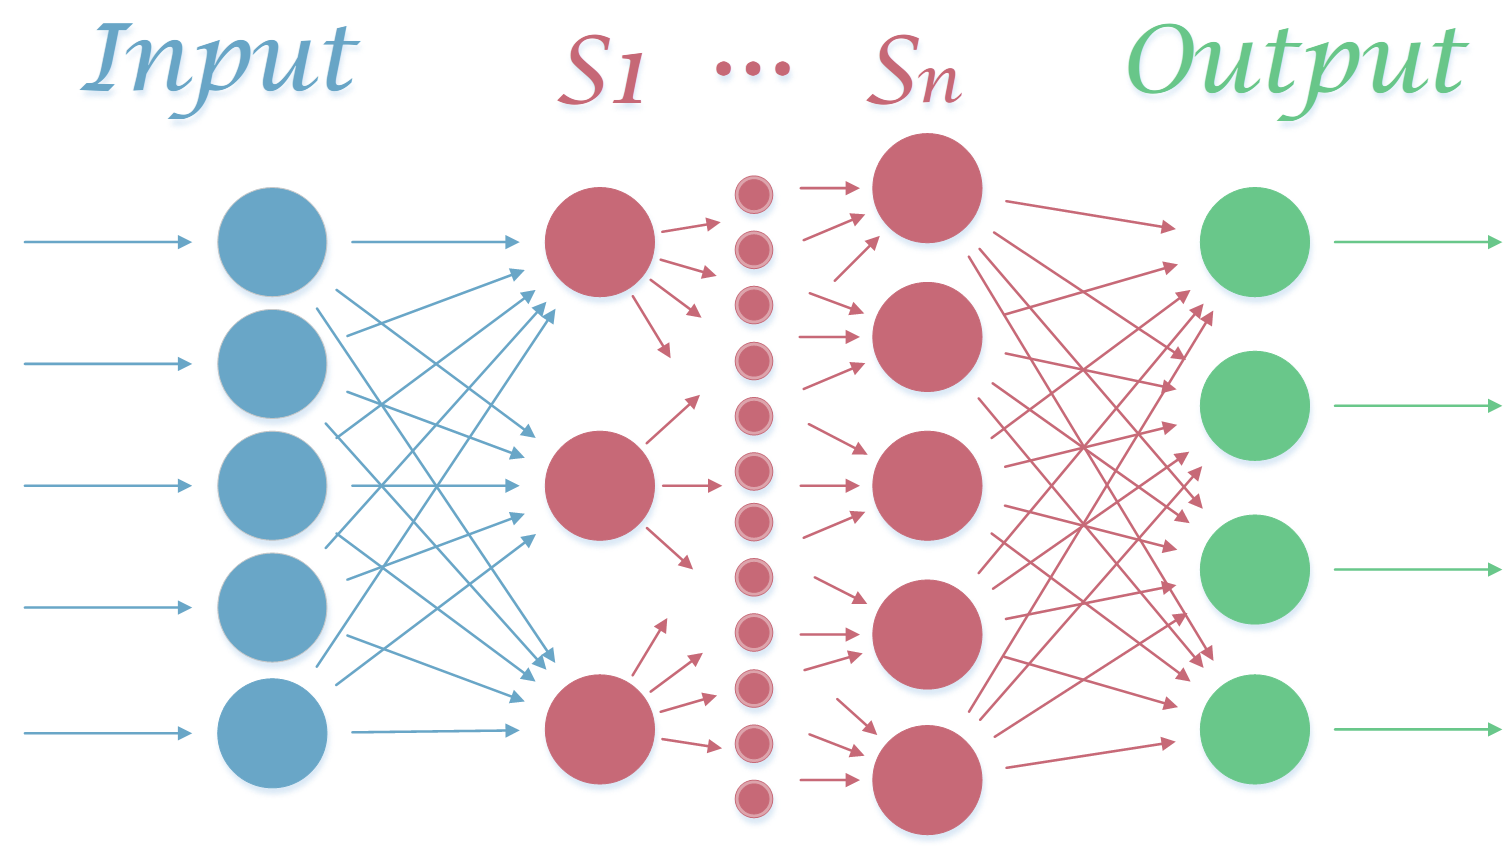
\includegraphics[height=4.4cm,width=3.1in]{pic/14.png}
\vspace{-1em}
\caption{深度学习数据处理流程}
\end{figure}
}

\frame {
\frametitle{深度学习自编码器}
\vspace{-0.5em}
\begin{columns}
\column{5cm}
\begin{figure}
\vspace{-0.5em}
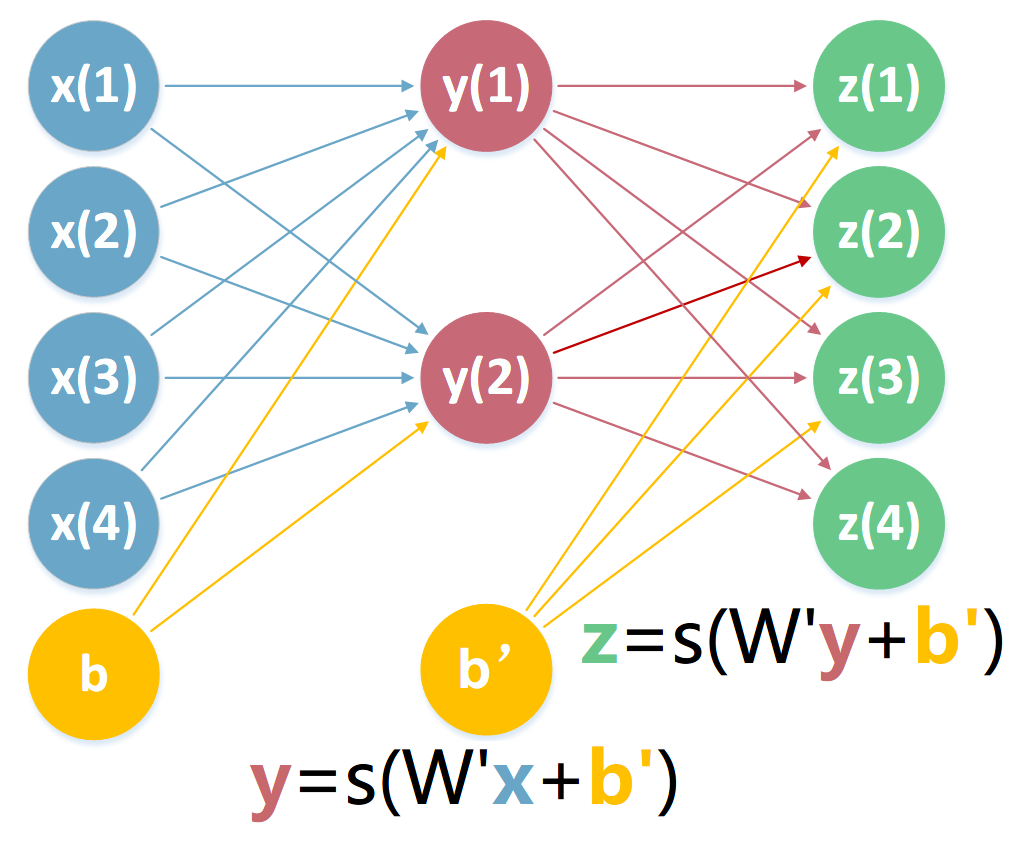
\includegraphics[height=5cm,width=5.8cm]{pic/15.png}
\vspace{-0.5em}
\caption{自编码器值传递流程}
\end{figure}
\column{5.3cm}
\begin{alertblock}{}
\begin{enumerate}
\item $s$是Sigmoid函数
\begin{equation}
s(x)=\frac{1}{1+e^{-x}}
\end{equation}
\item $W$是权重矩阵
\item $W'$是逆映射权重矩阵
\end{enumerate}
这个模型的目标便是优化得出平均重构误差最小的映射。
\begin{equation}
Argmin[L(xz)]=||x-z||^2
\end{equation}
\end{alertblock}
\end{columns}
}

\frame {
\frametitle{深度残差网络}
\begin{columns}
\column{5cm}
\begin{alertblock}{}
\qquad 深度残差网络解决了深度学习中精度下降的问题。

\qquad 假设深度神经网络的基础映射为 H(x),然后构造一个映射:
\begin{equation}
F(x)= H(x)-x
\end{equation}
\end{alertblock}
\column{5cm}
\begin{figure}
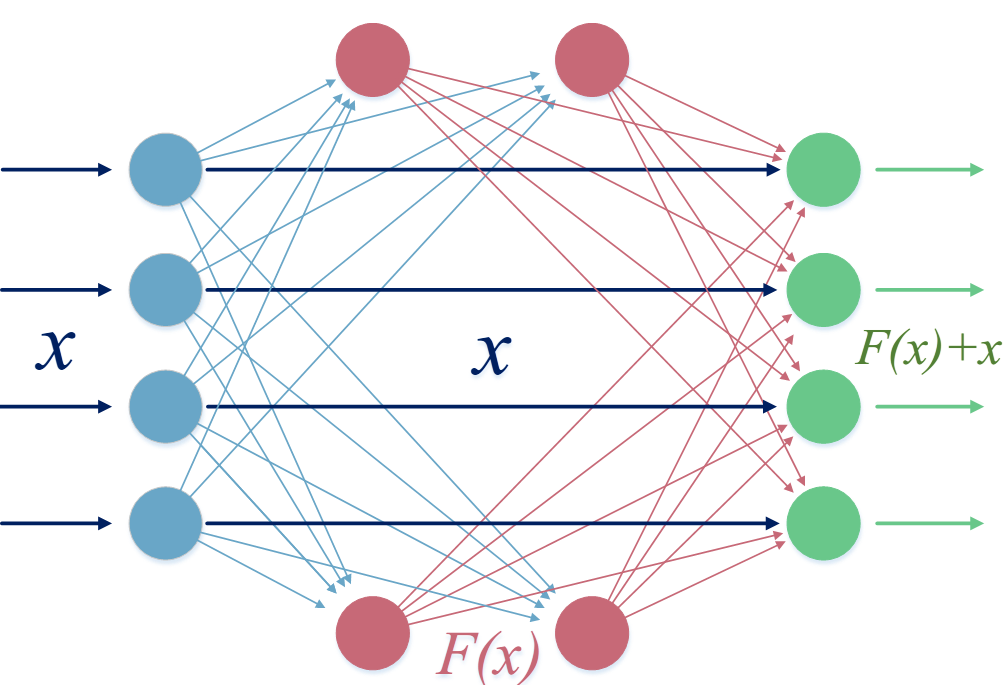
\includegraphics[height=4cm,width=2.1in]{pic/16.png}

\caption{深度残差网络值传递过程}
\end{figure}
\end{columns}
}


\subsection{数据的获取与预处理}
\frame {
\frametitle{国际金价历史数据的获取}
\begin{table}
\vspace{-2em}
\caption{原始数据(部分)的储存形式}
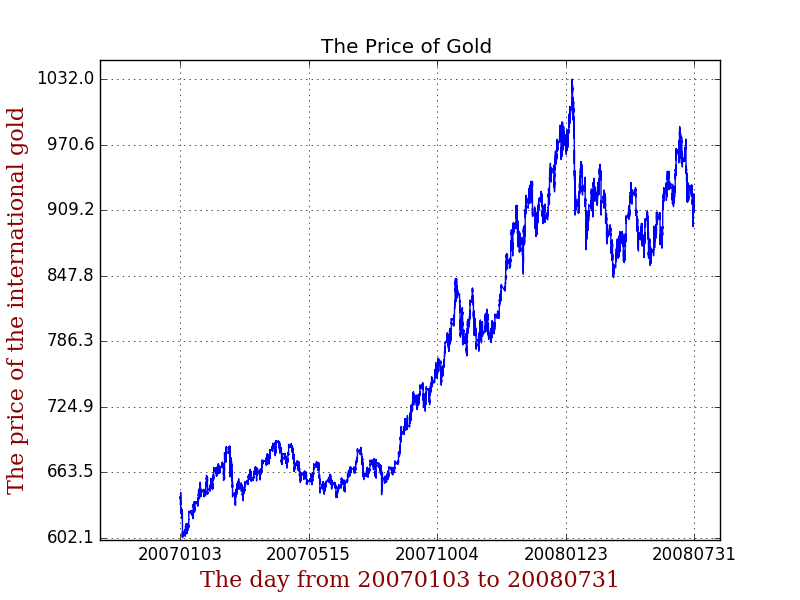
\includegraphics[height=2.6cm,width=4.5in]{pic/4.png}
\end{table}
\vspace{-1em}
\begin{columns}
\column{5cm}
通过Forextester网站可免费下载国际金价的历史数据。其数据以纯文本格式储存,提取其中的有用数据(黄色)并将时间转换为UTC格式。
\column{5cm}
\vspace{-1em}
\begin{table}
\caption{时间格式转换后的数据}
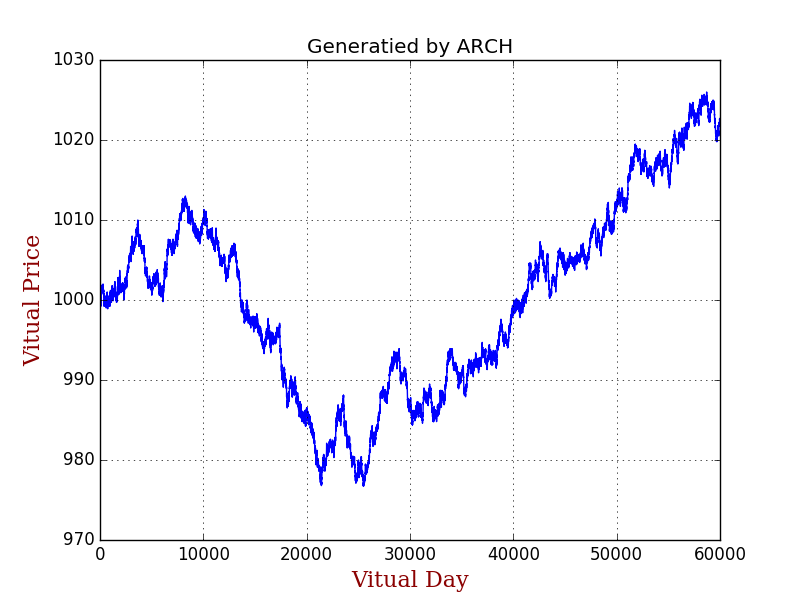
\includegraphics[height=2.5cm,width=4.5cm]{pic/5.png}
\end{table}
\end{columns}
}


\frame {
\frametitle{历史数据的预处理}
\begin{alertblock}{}
设$[i]$表示第i天对应的价格,且
\vspace{+0.8em}
\begin{columns}
\column{2.6cm}
$PMean$:均值\\$PMax$: 最大值\\$PMin$: 最小值
\column{6.7cm}
$LR$:10日平均对数收益率\\$XLR$:最大值的10日平均对数收益率\\$NALR$:最小值的10日平均对数收益率
\end{columns}
\end{alertblock}
\begin{table}
\vspace{-1em}
\caption{深度残差网络数据输入格式}
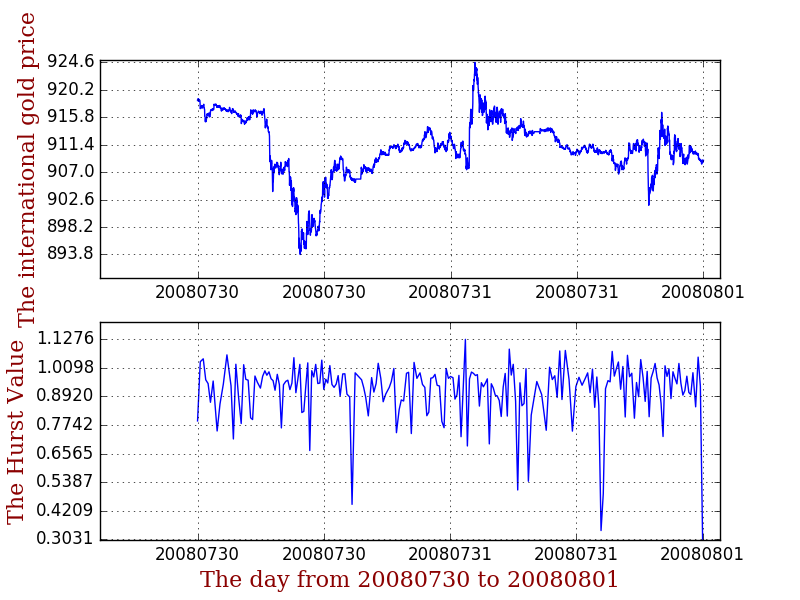
\includegraphics[height=2.1cm,width=4.3in]{pic/6.png}
\end{table}
}


\subsection{深度残差网络的搭建}
\frame {
\frametitle{深度残差网络的搭建环境}
在本实验的硬件条件下,深度残差网络总共训练161,000次,耗时约134小时。
\begin{table}
\vspace{-1.2em}
\caption{深度残差网络的搭建环境}
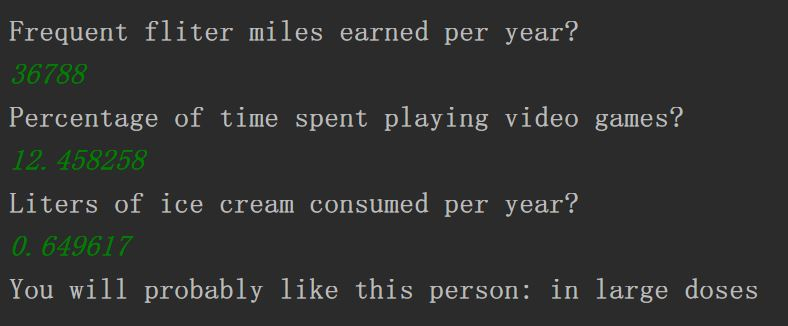
\includegraphics[height=4.2cm,width=3.7in]{pic/7.png}
\end{table}
}



\frame {
\frametitle{深度残差网络的训练过程}
\begin{columns}
\column{5cm}
\begin{alertblock}{判断预测准确性的规定}
\begin{enumerate}
\item 若某一日的预测与实际情况同为上涨或下跌,称为预测正确,否则称为预测不正确;
\item 若某一日的预测与实际情况同为大涨跌幅或小涨跌幅,称为涨跌幅预测正确,否则称为涨跌幅预测不正确。
\end{enumerate}
\end{alertblock}
\column{6cm}
\begin{figure}
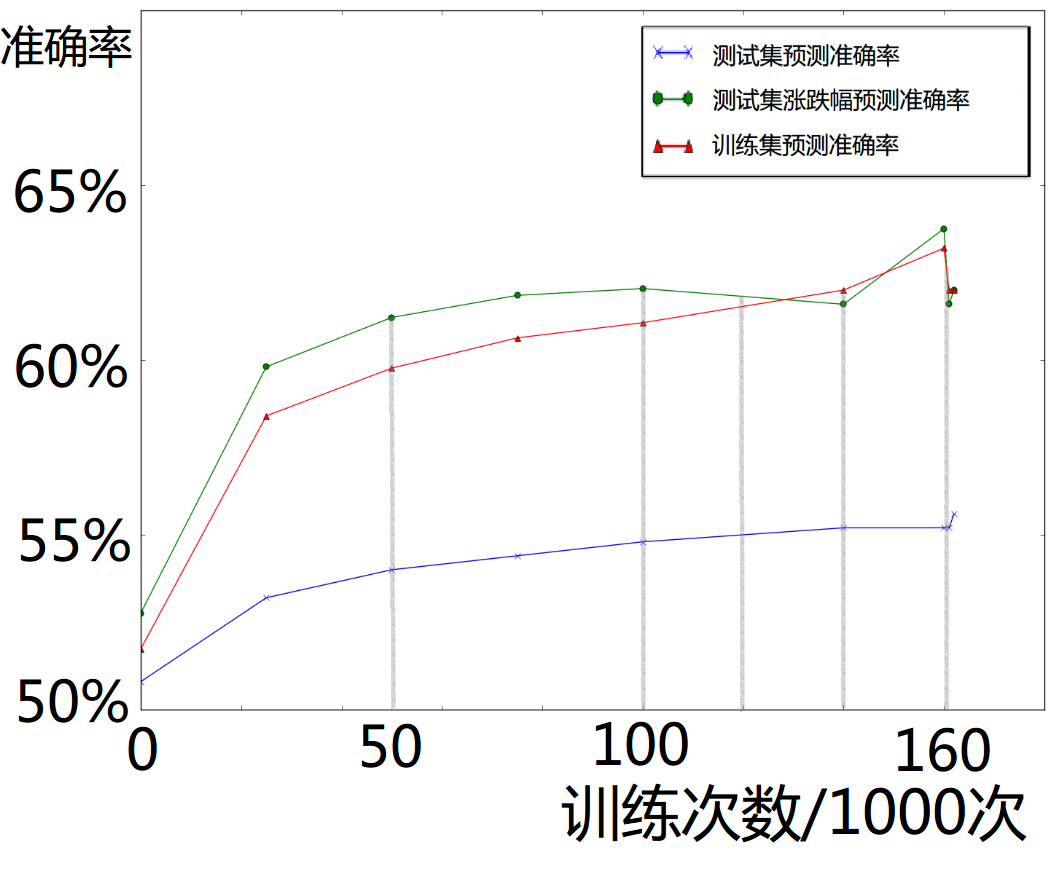
\includegraphics[height=5.6cm,width=2.4in]{pic/8.png}
\vspace{-1em}
\caption{训练的准确率变化曲线}
\end{figure}
\end{columns}
}


\frame {
\frametitle{深度残差网络的预测结果及分析}
利用训练完成的深度残差网络进行25交易日的金价走势。
\begin{figure}
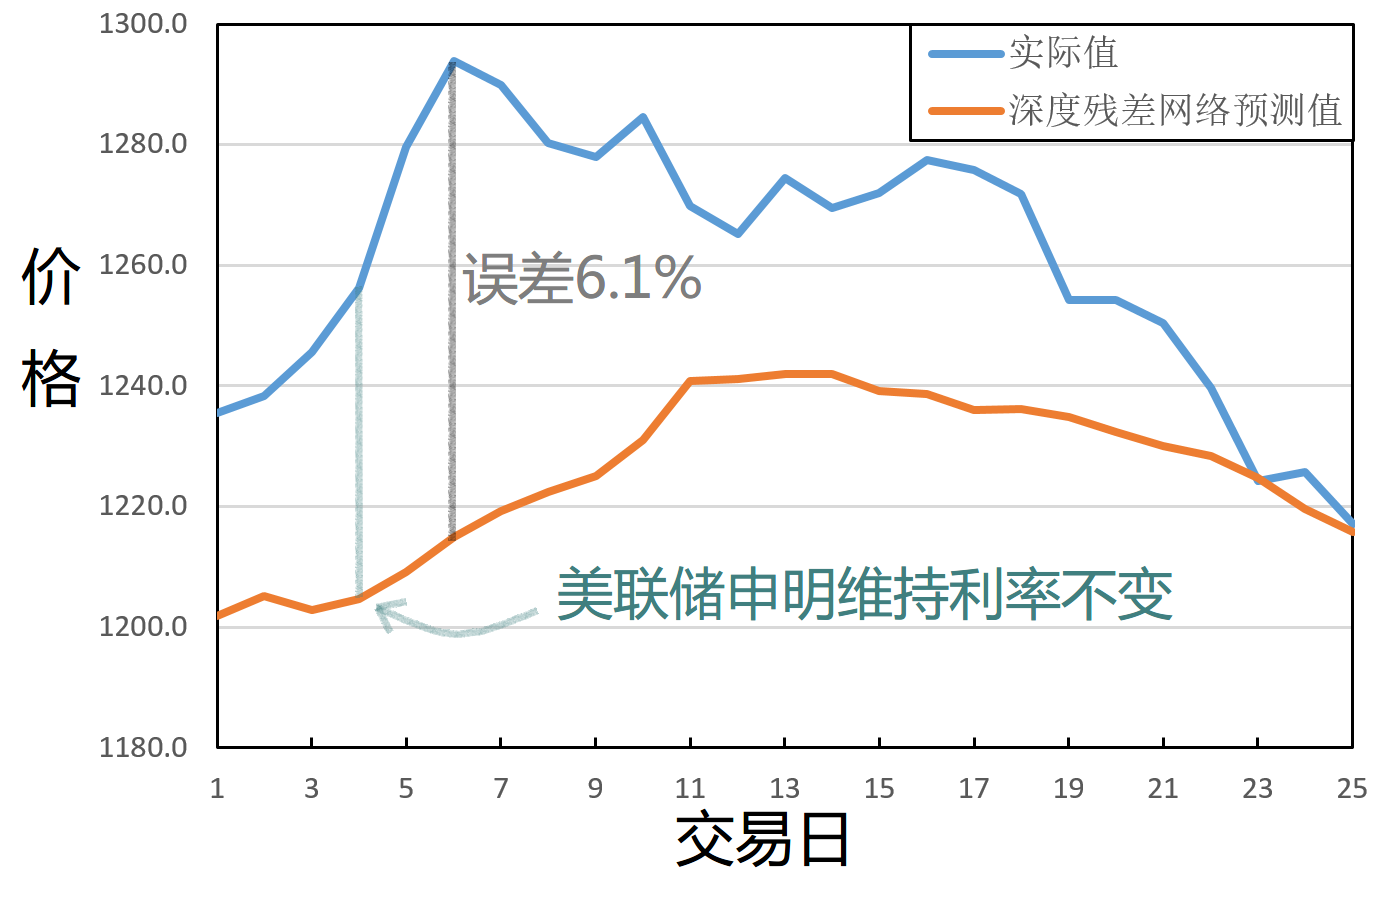
\includegraphics[height=5cm,width=3.45in]{pic/9.png}
\vspace{-1.2em}
\caption{2016年4月23日至5月27日预测结果}
\end{figure}
}


\section{专家系统}

\frame {
\frametitle{专家系统知识库的数据获取}
\vspace{-1.2em}
\begin{columns}
\column{4.6cm}
\begin{alertblock}{专家系统的数据来源}
\qquad 出于技术条件的限制,暂时使用“今日头条”门户网站的信息作为专家系统知识库的数据来源。

\qquad 爬虫软件将检测出“今日头条”搜索页面中的新闻网址链接并进行访问,然后将所有与“黄金”和“美元”相关的新闻备份至本地知识库。
\end{alertblock}
\column{5cm}
\begin{figure}
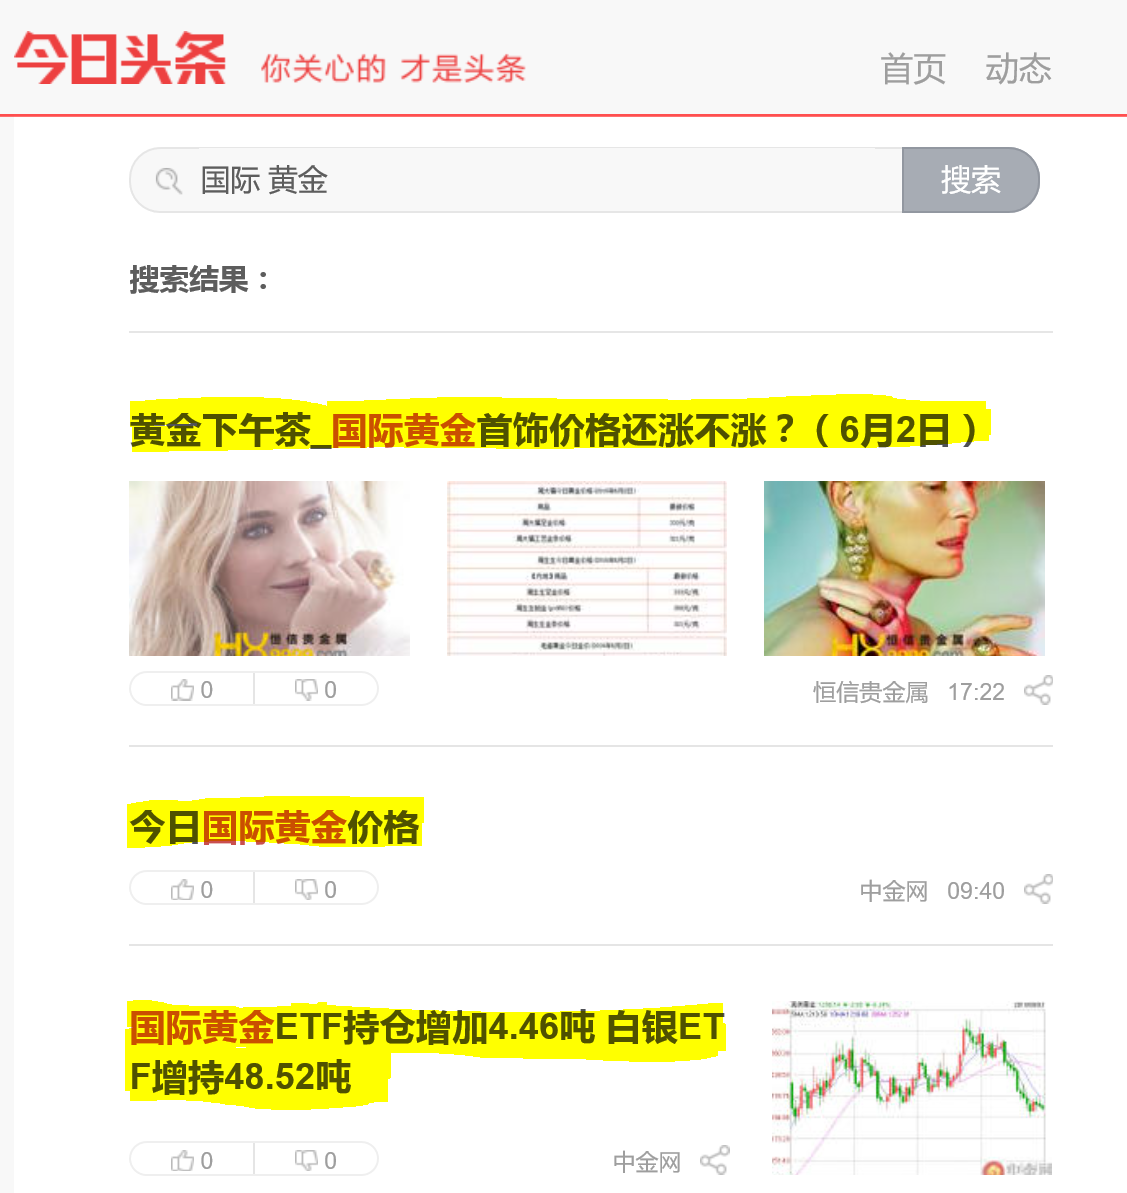
\includegraphics[height=6cm,width=2.2in]{pic/10.png}
\vspace{-1.2em}
\caption{今日头条搜索结果}
\end{figure}
\end{columns}
}


\frame {
\frametitle{专家系统推理库的设计}
专家系统对知识库中的信息进行分析和关键词提取。
\begin{figure}

\includegraphics[height=1.7cm,width=3.7in]{pic/11_1.png}

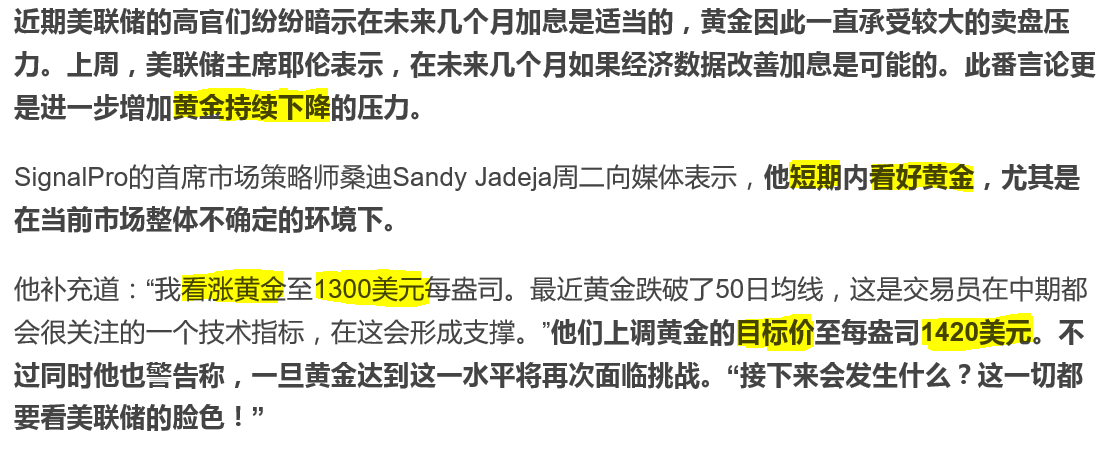
\includegraphics[height=3.6cm,width=3.7in]{pic/11_2.png}
\vspace{-1.2em}
\caption{推理库对关键词搜索结果}
\end{figure}
}

\frame {
\frametitle{专家系统推理库的设计}
\begin{alertblock}{}
\begin{columns}
\column{5.5cm}
\qquad 根据最大后验概率原理,确定权重系数 $k$:
\begin{equation}
k=\frac{(u-d)^2}{u+d}
\end{equation}
其中 $u$ 和 $d$ 分别表示预测金价上涨和下跌的关键词的出现次数。
\column{5.5cm}
然后计算得到修正后的金价 $CP$: 
\begin{equation}
CP=\frac{kD+P}{1+k}
\end{equation}
其中 $D$ 表示推理库的预测值,$P$ 表示深度残差网络的预测值。
\end{columns}
\end{alertblock}
\begin{table}
\vspace{-1.2em}
\caption{专家系统5月24日至5月26日知识库数据}
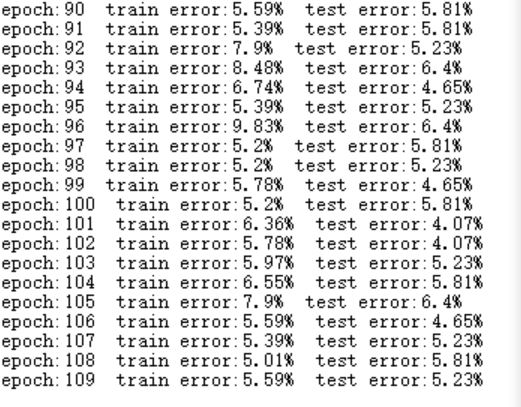
\includegraphics[height=1.95cm,width=3.8in]{pic/12.png}
\end{table}
}




\frame {
\frametitle{专家系统的修正结果与分析}
我们利用专家系统推理库对25交易日的金价预测结果进行修正。
\begin{figure}
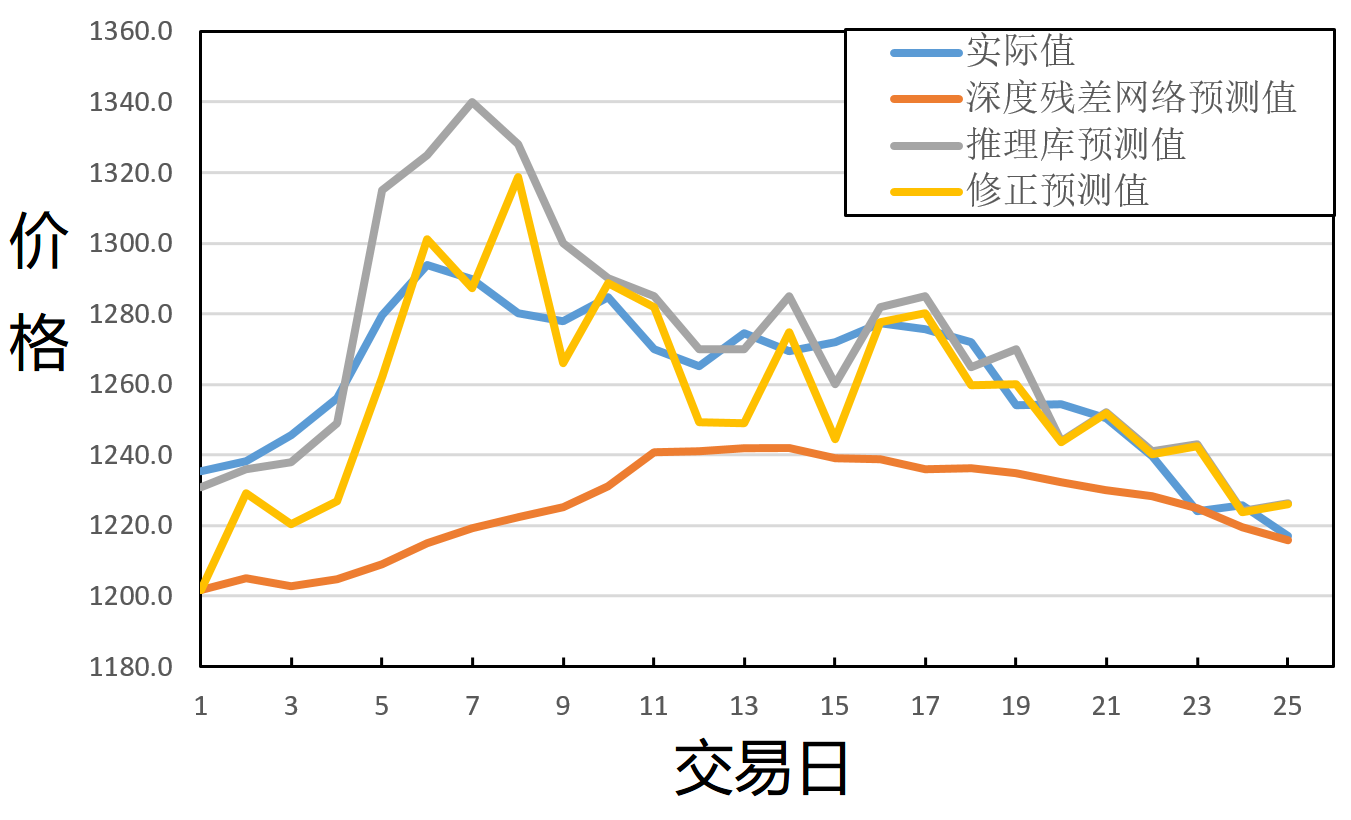
\includegraphics[height=5.1cm,width=3.4in]{pic/13.png}
\vspace{-1.2em}
\caption{推理库修正预测值与深度残差网络预测值对比}
\end{figure}
}

\frame {
\frametitle{专家系统的修正结果与分析}
\begin{alertblock}{结果分析}
\qquad 深度残差网络预测均方误差(误差平方的均值)为1682.7,专家系统推理库预测均方误差为370.6,深度残差网络加权修正预测均方误差为292.8。

\qquad 深度残差网络预测了国际金价市场的内部规律,专家系统提供对于国际金融事件的应变能力,两者互补得到预测均方误差最小的加权修正预测值。
\end{alertblock}
}



\section{总结}
\frame {
\frametitle{总结}
\begin{alertblock}{}
\begin{enumerate}
\item 在规定时间内完成了课题所要求的全部任务。
\item 总共编写超过2000行Python代码,编程能力有了一定的突破,对Python编程语言有了更深的理解。
\item 查阅深度学习、国际金融学大量书籍,对于计算机科学和经济学有了更深的认识和学习兴趣。
\item 知识整合能力得到提升, 在整个课题中, 运用不同平台下各种工具综合解决问题。
\end{enumerate}
\end{alertblock}
}

\frame {
\frametitle{展望}
\begin{alertblock}{}
\begin{enumerate}
\item 利用纯粹的深度算法进行金融市场的预测研究不建议继续进行。
\item 专家系统的预测准确性极高,值得进一步的研究。可以尝试从增加专家系统搜索关键词的数量、增加门户网站的搜索数量等方面,提高专家系统知识库的覆盖面。
\item 可以考虑利用深度学习结合专家系统的爬虫软件,进行“智能”的数据挖掘。
\item 专家系统可以考虑支持多语言的数据处理。
\end{enumerate}
\end{alertblock}
}

\frame {
\frametitle{致谢}
\centerline{\Large{感谢各位的聆听! 请各位老师给予批评和指导!}}
}
\end{document}